\RequirePackage[final]{graphicx}
\documentclass[a4paper,12pt,draft]{article}
\usepackage[T2A]{fontenc}
\usepackage[english,russian]{babel}
\usepackage[utf8]{inputenc}
\usepackage[indentfirst,compact,topmarks,calcwidth,pagestyles]{titlesec}
\usepackage{graphicx}
\graphicspath{{pictures/}}
\DeclareGraphicsExtensions{.png,.pdf}

\usepackage{array}

\usepackage{setspace}
\setstretch{1.15}

\usepackage{lastpage}

\usepackage{fancyhdr}

\usepackage{censor}
\StopCensoring

\usepackage{hyperref}

\usepackage{comment}

\usepackage{geometry} % Меняем поля страницы
\geometry{left=3cm}% левое поле
\geometry{right=1.5cm}% правое поле
\geometry{top=2cm}% верхнее поле
\geometry{bottom=3cm}% нижнее поле

\begin{document}

%\section{Запуск конфигурации}
%\section{Основное рабочее пространство}
\section{Заполнение справочных данных}

\subsection{Регистр сведений <<Учетная ставка>>}
В данном регистре хранятся сведения об учетной ставке Банка России (до 01 января 2016 года --- ставка рефинансирования, с 01 января 2016 года --- ключевая ставка).
\begin{figure}[h]
\center{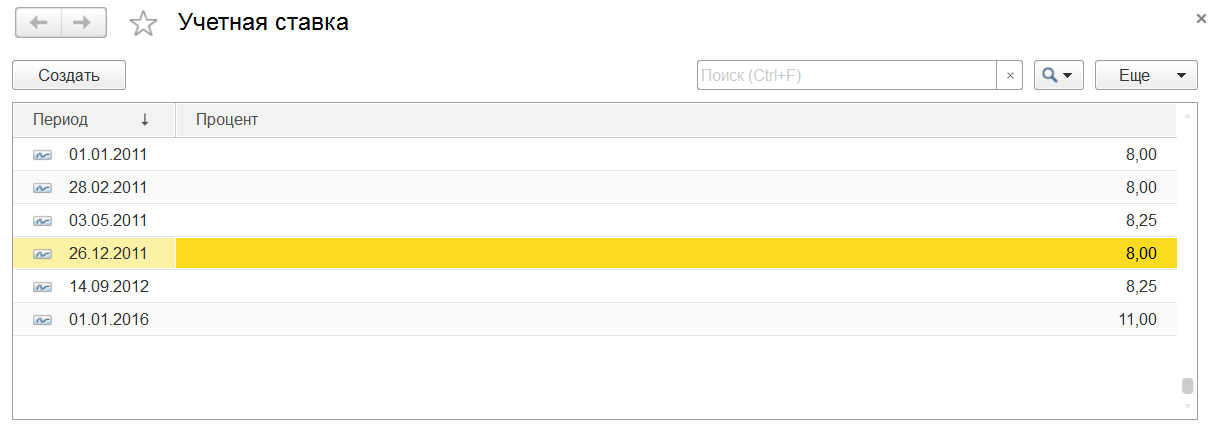
\includegraphics[scale=0.5]{rs_uch}}
\caption{Регистр сведений <<Учетная ставка>>}
\label{ris:rs_uch}
\end{figure}

Данная ставка утверждается Банком России и является базой для расчета процентной ставки пени за несвоевременную уплату взносов на капитальный ремонт, жилищные и коммунальные услуги, а также она применялась как ставка для расчета процентов за пользование денежными средствами (в периоды до 01 июня 2015 года).
\subsection{Регистр сведений <<Средняя ставка банковского процента по вкладам физлиц>>}
Согласно изменениям в статью 395 Гражданского Кодекса РФ, с 01 июня 2015 года для расчета сумм процентов за пользование денежными средствами применяется средняя ставка банковского процента по вкладам физических лиц, регулярно публикуемая Банком России
\begin{figure}[h]
\center{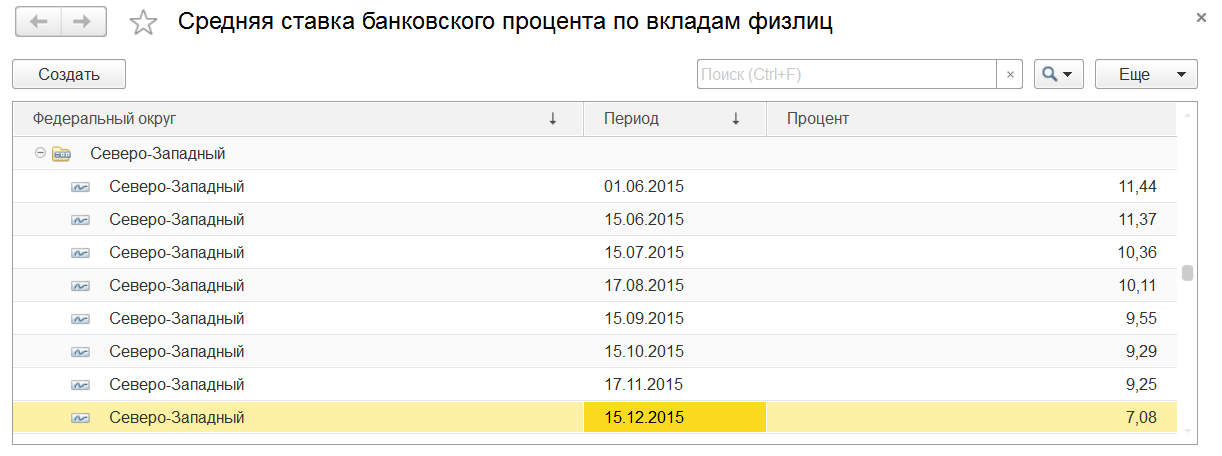
\includegraphics[scale=0.5]{rs_fl}}
\caption{Регистр сведений <<Средняя ставка банковского процента по вкладам физлиц>>}
\label{ris:rs_fl}
\end{figure}

Аналогично коэффициентам индексации, данные процентные показатели не являются общими для всей территории РФ, а детализируются до уровня федерального округа. Поэтому с целью удобства работы с регистром, показатели в нём сгруппированы по федеральным округам, и сама таблица с содержимым регистра представляет собой двухуровневое дерево.
\clearpage
\section{Документ <<Неустойка по алиментам>>}

\parindent=1cm

Неустойка за несвоевременную уплату алиментов является мерой семейно-пра\-во\-вой ответственности, предусмотренной ч. 2 ст. 115 Семейного Кодекса РФ. Взыскание данной неустойки производится с лица, обязанного по судебному решению производить уплату алиментов, но по собственной вине не производящего уплату.

\subsection{Предварительные требования}
В настоящий момент точный и подробный алгоритм расчета неустойки федеральным законодательством и/или постановлениями высших судов не утвержден. Однако, в силу данных ВС РФ актуальных разъяснений\footnote{<<Обзор судебной практики по делам, связанным со взысканием алиментов на несовершеннолетних детей, а также на нетрудоспособных совершеннолетних детей>> (утвержден Президиумом Верховного Суда РФ 13 мая 2015 года), раздел X} расчет неустойки должен производиться дифференцированно --- исходя из каждого платежа по сроку и с учетом погашения задолженности, пусть даже если оно было частичным.

В подавляющем большинстве случае задолженность должника по алиментам, на которую начисляется неустойка, рассчитывается исходя из определенной доли среднего заработка по РФ.

Первичным документом для расчета в таком случае является постановление судебного пристава-исполнителя о расчете задолженности по алиментам\footnote{ч. 2, 3 ст. 102 Федерального закона от 02.10.2007 г. № 229-ФЗ <<Об исполнительном производстве>>, п. 5.1 <<Методических рекомендаций по порядку исполнения требований исполнительных документов о взыскании алиментов>> (утверждены ФССП России 19.06.2012 г. за № 01-16)}.
Для правильного исчисления постановление должно содержать следующие сведения:
\begin{enumerate}
\item сумму начальной (входящей) задолженности --- в случае, если расчет задолженности производится не с даты назначения алиментов и на дату начала расчета у должника уже сформирована некая задолженность; в противном случае размер задолженности принимается равным нулю;
\item набор периодов расчета задолженности с суммой задолженности за каждый период\label{Periody};
\item суммы оплат, произведенных должником в расчетном периоде (в случае, если оплаты производились).
\end{enumerate}

Далее, если в периоде расчета задолженности из пункта~\ref{Periody} ответчиком была произведена оплата, то период расчета задолженности делится на два подпериода --- по дату, предшествующую дате оплаты, и начиная с даты оплаты; при этом для целей расчета задолженности сумма оплаты относится к первому подпериоду\footnote{Это сделано с целью недопущения нарушения интересов ответчика --- для расчета считается, что с даты оплаты он погасил задолженность на сумму, равную сумме оплаты}. Если в периоде было несколько оплат --- это деление производится необходимое число раз.

Если один из периодов содержит дату 01 января 2008 года --- дату изменения расчетного процента неустойки --- то производится аналогичное деление, как если бы 01 января 2008 года ответчик произвел бы оплату (но без суммы).

Отдельно необходимо обратить внимание на то, что периоды, указанные в пункте~\ref{Periody}, в обязательном порядке должны быть смежными, т.е. дата начала следующего периода расчета должна следовать за датой окончания предыдущего. Если это требование не соблюдено, то необходимо последовательно проводить расчет неустойки несколько раз, каждый раз исчисляя сумму задолженности на начало периода, а затем суммировать суммы рассчитанной неустойки за все периоды.

Итоговый алгоритм расчета неустойки выглядит таким образом:
\begin{enumerate}
    \item Для самого первого периода размер задолженности на начало устанавливается в размере входящей задолженности из постановления;
    \item Размер задолженности на конец периода устанавливается по формуле: {\it задолженность на конец = задолженность на начало + начислено в периоде - оплачено в периоде};
    \item Для всех периодов, начиная со второго, размер задолженности на начало устанавливается в размере задолженности на конец по предшествующему ему периоду;
    \item Для каждого из периодов производится подсчет количества календарных дней, в него входящих (включая границы периода);
    \item Если на начало периода задолженность на начало положительна, то рассчитывается неустойка за день (умножением суммы задолженности на начало на действующую в данном периоде процентную ставку), которая затем умножается на количество дней и дает в итоге размер неустойки за этот период;
    \item Итоговая неустойка по расчету вычисляется суммированием всех неустоек, рассчитанных по подпериодам.
\end{enumerate}

Дополнительно необходимо отметить, что в последнем периоде расчета неустойка исчисляется исходя из сформированной задолженности на начало периода расчета; таким образом, сумма начисления за последний расчетный период сама по себе для расчета не учитывается (что логично, так как срок оплаты для этой начисленной сумме в нашем расчетном периоде не наступил и de jure долгом она ещё не является).
\subsection{Регистр сведений <<Процент неустойки по алиментам>>}
Для правильного расчета неустойки в обязательном порядке должна быть заполнена хронология применяемых процентных ставок неустойки --- регистр сведений <<Процент неустойки по алиментам>>.

В данном регистре хранится процентная ставка за день, применяемая для расчета неустойки за неуплату алиментов в срок, предусмотренной статьей 155 СК РФ. 
\begin{figure}[h]
\center{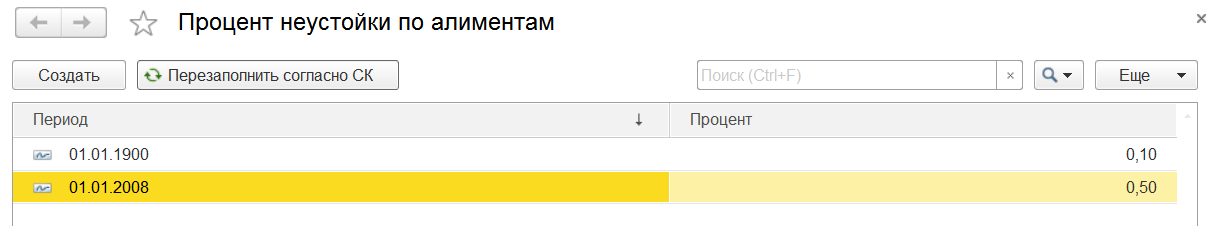
\includegraphics[scale=0.5]{razm_neus}}
\caption{Регистр сведений <<Процент неустойки по алиментам>>}
\label{ris:razm_neus}
\end{figure}

Регистр заполнен по умолчанию согласно законодательству с учетом его изменений в прошлом, а именно:
\begin{itemize}
\item В периоды до 01 января 2008 года --- в размере 0,1\% от суммы задолженности;
\item С 01 января 2008 года --- в размере 0,5\% от суммы задолженности.
\end{itemize}

В случае, если в будущем процентная ставка неустойки будет изменена --- в регистр могут вноситься дополнительные записи, действующие с указанной даты.

Если в регистр внесены ошибочные записи, либо, наоборот, удалены правильные --- он всегда может быть приведен в изначальное (соответствующее изменениям СК РФ) состояние нажатием кнопки <<{\it Перезаполнить согласно СК}>>
\subsection{Пример, используемый для заполнения документа}
\label{sec:neus}
Истец Иванова обратилась к мировому судье с иском на предмет взыскания не\-ус\-тойки по алиментам с бывшего мужа Петрова за период с 02~февраля 2014 года по 08~декабря 2014 года.

В обоснование своих требований истец представила решение мирового судьи о назначении алиментов и постановления судебного пристава-исполнителя о расчете задолженности по алиментам.

Согласно представленным документам, сформированная задолженность по алиментам на 02 февраля 2014 года --- дату начала расчета --- составила 86~916~рублей 18~копеек.

Далее, за период, указанный в иске, судебным приставом была исчислена задолженность в общей сумме 82~890~рублей 90~копеек, согласно постановлению разделенная на периоды (таблица \ref{tab:neus}):



\begin{table}[h]
\begin{center}
\begin{tabular}{|r|r|r|r|}
\hline
\bf № п/п&\bf Начало периода&\bf Конец периода&\bf Начислено\\
\hline
1&02 февраля 2014&02 марта 2014&7 754-31\\
\hline
2&03 марта 2014&02 апреля 2014&8 289-09\\
\hline
3&03 апреля 2014&02 мая 2014&8 021-70\\
\hline
4&03 мая 2014&02 июня 2014&8 289-09\\
\hline
5&03 июня 2014&02 июля 2014&8 021-70\\
\hline
6&03 июля 2014&02 августа 2014&8 289-09\\
\hline
7&03 августа 2014&02 сентября 2014&8 289-09\\
\hline
8&03 сентября 2014&02 октября 2014&8 021-70\\
\hline
9&03 октября 2014&02 ноября 2014&8 289-09\\
\hline
10&03 ноября 2014&08 декабря 2014&9 626-04\\
\hline
\end{tabular}
\end{center}
\caption{Начисления по периодам}
\label{tab:neus}
\end{table}

В спорном периоде должником были произведены две оплаты на общую сумму 54~000~рублей --- 12 февраля 2014 года на сумму 14~000~рублей и 07 марта 2014 года на сумму 40 000 рублей.
\subsection{Последовательность заполнения документа}

Основное окно документа, заполненного согласно примеру из раздела \ref{sec:neus}, представлено на рисунке \ref{ris:neus}.
\begin{figure}[h]
\center{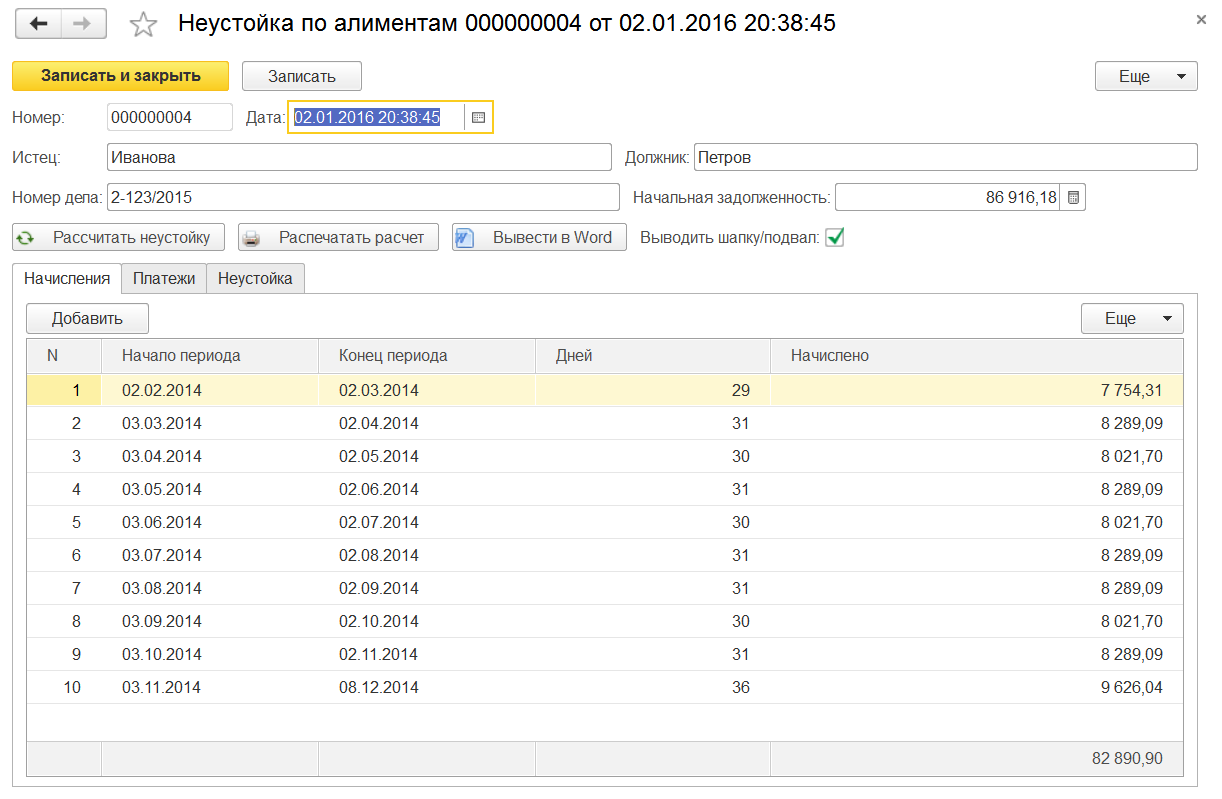
\includegraphics[scale=0.5]{Neus1}}
\caption{Окно документа <<{\it Неустойка по алиментам}>>}
\label{ris:neus}
\end{figure}

Поля <<{\it Номер}>> и <<{\it Дата}>> заполняются автоматически, при этом номер документа присваивается последовательно, а дата выставляется равной текущей дате. При необходимости эти поля можно отредактировать вручную, но обязательным это не является.

Заполнение полей <<{\it Истец}>>, <<{\it Должник}>> и <<{\it Номер дела}>> не является строго обязательным, однако рекомендуется --- при заполнении эти поля будут автоматически внесены в печатную форму расчета и выведены в отдельные графы при просмотре списка всех введенных документов, что облегчит ориентирование при их большом количестве.

В поле <<{\it Начальная задолженность}>> вносится сумма задолженности по алиментам, сформированная на дату начала расчета неустойки. В случае, если неустойка рассчитывается с даты назначения алиментов или ранее алименты уплачивались в срок, это поле не заполняется и принимается для расчета равным нулю.

Затем заполняется таблица на вкладке <<{\it Начисления}>>. Заполнение производится построчно, заполняются графы <<{\it Начало периода}>>, <<{\it Конец периода}>> и <<{\it Начислено}>>. При этом графа <<{\it Дней}>> заполняется автоматически количеством календарных дней между началом и концом периода, включая эти даты, а в итоговой строке таблицы выводится общая сумма начисления за период, которую можно сверить с постановлением о расчете задолженности.

Далее, если должником производились оплаты в расчетном периоде, то они вносятся в таблицу на вкладке <<{\it Платежи}>> (рисунок \ref{ris:opl}).
\begin{figure}[h]
\center{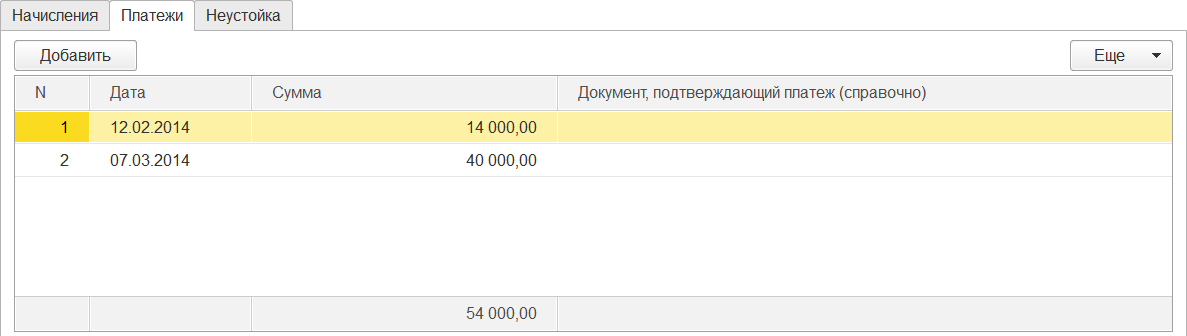
\includegraphics[scale=0.5]{Neus2}}
\caption{Таблица <<{\it Платежи}>>}
\label{ris:opl}
\end{figure}

Обязательным является заполнение граф <<{\it Дата}>> и <<{\it Сумма}>>, а в графу <<{\it Документ, подтверждающий платеж (справочно)}>> рекомендуется вносить реквизиты подтверждающего оплату документа --- платежного поручения либо постановления судебного пристава-исполнителя о распределении взысканных сумм. При этом в целях сверки в низ таблицы выводится итоговая сумма всех внесенных оплат.

В случае, если в таблицы документа внесены все необходимые сведения, можно произвести расчет нажатием кнопки <<{\it Рассчитать неустойку}>>. При этом заполняется сводный расчет на вкладке <<{\it Неустойка}>> (рисунок \ref{ris:itog}).

\begin{figure}[h]
\center{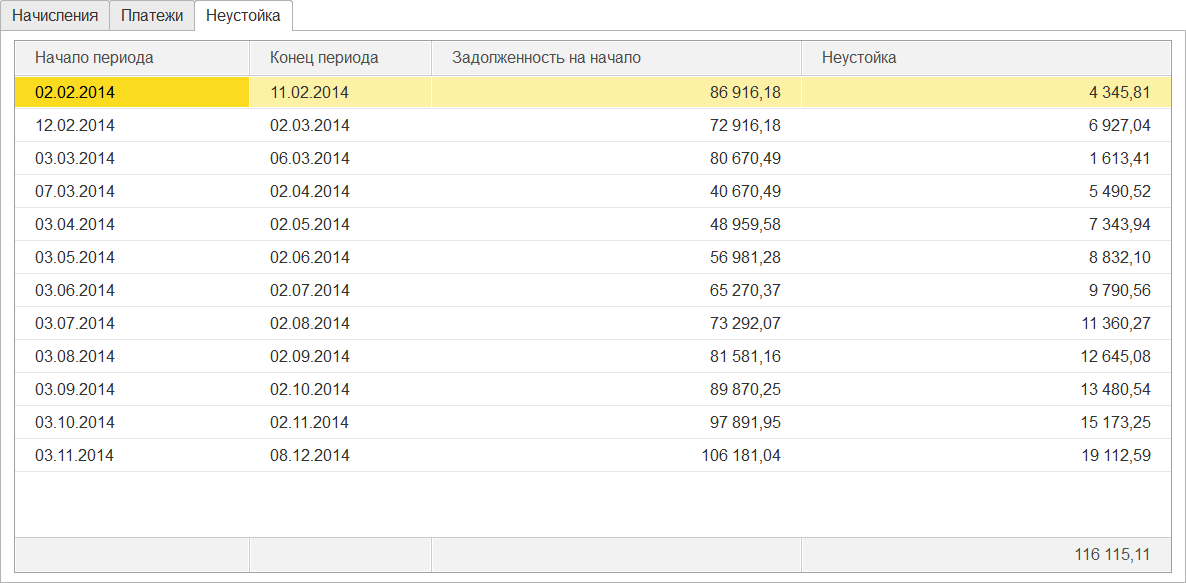
\includegraphics[scale=0.5]{Neus3}}
\caption{Таблица <<{\it Неустойка}>>}
\label{ris:itog}
\end{figure}

Справочно в низ таблицы выведен итог по графе <<{\it Неустойка}>>.

Следует обратить внимание на два момента:
\begin{enumerate}
\item Таблица неустойки недоступна для редактирования пользователем --- её заполнение производится только автоматически на основании данных в таблицах <<{\it Начисления}>> и <<{\it Платежи}>>;
\item В случае, если после расчета неустойки данные о начислениях и/или платежах были изменены, расчет нажатием кнопки <<{\it Рассчитать неустойку}>> должен быть произведен повторно\footnote{Возможность автопересчета неустойки при внесении изменений в таблицы документа запланирована для реализации в будущем}.
\end{enumerate}

После того, как расчет произведен и таблица <<{\it Неустойка}>> заполнена, становится возможным вывести печатную форму расчета в удобном для редактирования и/или печати виде. Для этого предназначены кнопки <<{\it Распечатать расчет}>> и <<{\it Вывести в Word}>>. В зависимости от того, которую из кнопок выбрал пользователь:
\begin{enumerate}
\item Таблица с детальным расчетом будет выведена во встроенном табличном редакторе системы 1С
\item[] либо
\item Таблица с детальным расчетом будет открыта в установленном на компьютере пользователя редакторе Microsoft Word\footnote{Точнее, будет вызвано приложение, на конкретном компьютере ассоциированное с расширением файлов {\bf *.docx}}.
\end{enumerate}

Образец печатной формы расчета приведен на рисунке \ref{ris:pf}:
\begin{figure}[th]
\center{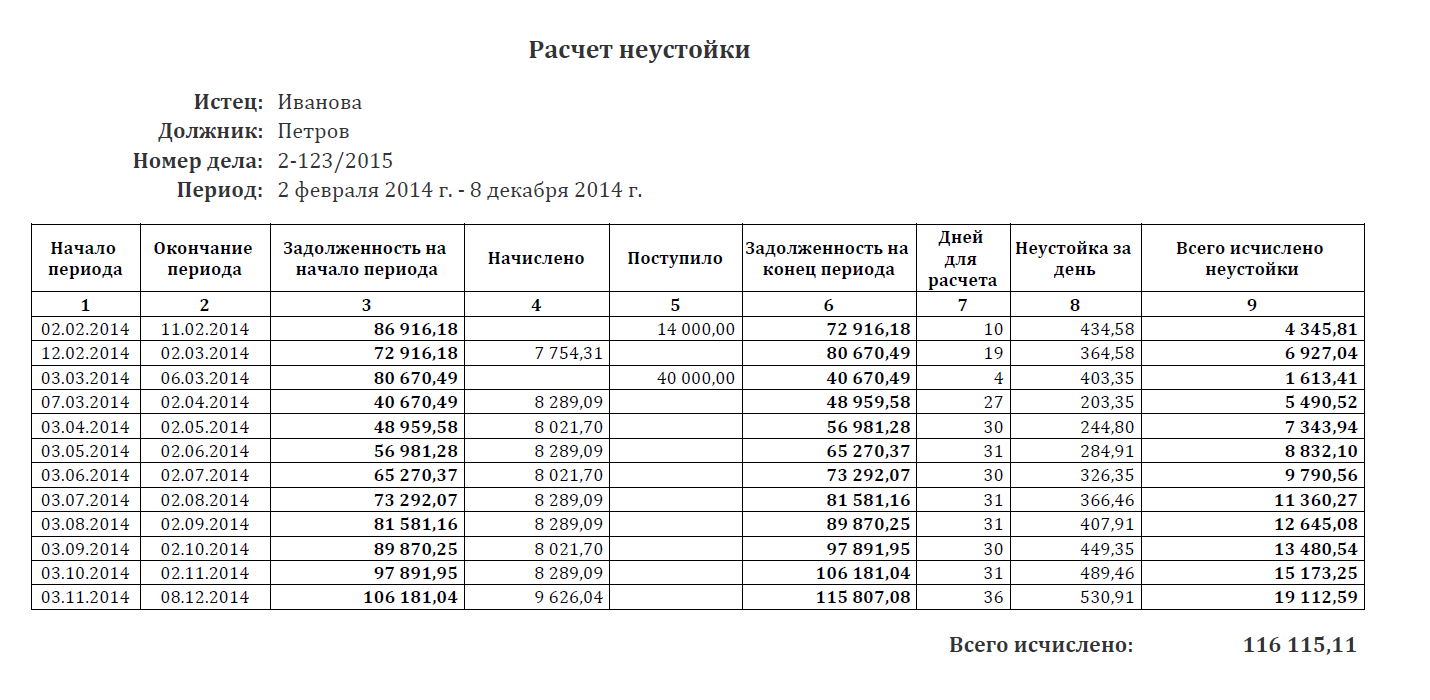
\includegraphics[scale=0.5]{Obr2}}
\caption{Итоговый расчет для печати}
\label{ris:pf}
\end{figure}

Вывод заголовка формы с реквизитами не является обязательным --- он производится в зависимости от того, установлен ли в форме документа флажок <<{\it Выводить шапку/подвал}>>. По умолчанию данный флажок включен.
\clearpage
\section{Документ <<Индексация присужденных сумм>>}

В случае, если исполнение судебного решения, оцененного в денежной форме, не производится вовремя, взыскатель имеет право произвести индексацию присужденных сумм (ст. 208 ГПК РФ).

Данная мера направлена на сохранение ценности присужденной суммы в условиях инфляционных процессов, постоянно обесценивающих денежную массу.

Моментом присуждения, согласно позиции высшего суда\footnote{Обзор судебной практики Верховного Суда Российской Федерации № 1 за 2015 год (утвержден Президиумом Верховного Суда Российской Федерации 04 марта 2015 года), пункт 9}, является дата вынесения судебного решения. Далее, минимальный временной интервал, отсчитываемый с даты вынесения решения, по истечении которого судебное решение для целей применения ст. 208 ГПК РФ, считается неисполненным, законодательно не установлен; следовательно, индексация присужденных сумм может исчисляться начиная с даты\footnote{Вопрос включения в расчетный период для расчета индексации самой даты вынесения решения является открытым}, следующей за датой вынесения судебного решения.

Как и для случая расчета неустойки по алиментам, четкий формальный алгоритм расчета сумм индексации законодательно не установлен. Дополнительно к этому, при расчете необходимо соблюсти баланс интересов сторон, а именно --- учесть, что судебное решение может исполняться должником частично неполными суммами. Более того, процессуальное законодательство не содержит запрета взыскателю обращаться за индексацией судебного решения неоднократно, что тоже должно быть учтено при расчете.

При расчете суммы индексации необходимо применять средневзвешенные коэффициенты роста потребительских цен, установленные уполномоченным органом --- территориальным подразделением Федеральной службы государственной статистики --- для субъекта Федерации, в котором находится взыскатель. Однако нужно принять во внимание, что приведенные там коэффициенты выведены в процентах и для целей расчета должны быть поделены на 100 (например, если на сайте коэффициент указан, как 104,3\%, то для расчета нужно использовать величину 1,043)

\begin{comment}
Для общего случая формула расчета проиндексированной суммы судебного решения имеет следующий вид:
\begin{equation}
\label{form:ind1}
S=S_0\times\prod_{n=1}^{m}\left(1+\frac{d^*_n}{d_n}\left(k_n-1\right)\right),
\end{equation}
или, в более удобном для расчета только суммы индексации виде:
\begin{equation}
\label{form:ind2}
I=S-S_0=S_0\times\left(\prod_{n=1}^{m}\left(1+\frac{d^*_n}{d_n}\left(k_n-1\right)\right)-1\right),
\end{equation}
где $I$ --- собственно сумма индексации, $S_0$ --- первоначальная сумма судебного решения, $S$ --- сумма решения с учетом индексации, $k_1, k_2,\dots, k_m$ --- коэффициенты индексации в каждом из месяцев, начиная от даты присуждения сумм и до момента, по который производится индексация, $d_1, d_2,\dots,d_m$ --- продолжительность месяца, входящего в период расчета, в календарных днях, $d^*_1, d^*_2,\dots,d^*_m$ --- соответственно, количество календарных дней, входящих в данных месяцах в период расчета.

Следует помнить, что из (\ref{form:ind2}) следует, что в общем случае индексация судебного решения за некоторый период не может быть точно вычислена сложением сумм индексации за подпериоды --- выражение для индексации не обладает свойством аддитивности.
% Для полного понимания разницы между $d$ и $d^*$ следует отметить, что если месяц входит в расчетный период полностью, то множитель $\displaystyle\frac{d^*_n}{d_n}$ за этот месяц будет равен единице, а выражение внутри знака произведения сократится до одного члена $k_n$, что соответствует порядку расчета коэффициента роста потребительских цен за несколько последовательных месяцев, приведенному на сайте ТОГС.
\end{comment}
Для случая, когда в период расчета сумм индексации должником проводилось частичное исполнение судебного решения, индексация рассчитывается отдельно за каждый период между оплатами исходя из суммы судебного решения за вычетом ранее исполненных сумм, а итоговая индексация принимается\footnote{Говоря строго, сумма индексации за период не точно, а приближенно равна сумме индексаций за входящие в него периоды; однако, при условии, что коэффициенты индексации приблизительно равны единице --- сумма погрешности несущественна} равной сумме всех рассчитанных индексаций за данные подпериоды.
\subsection{Регистр сведений <<Коэффициенты индексации>>}
\label{sec:rs_ind}
Для правильного расчета необходимо заполнение хранилища коэффициентов индексации --- одноименного регистра сведений.
\begin{figure}[h]
\center{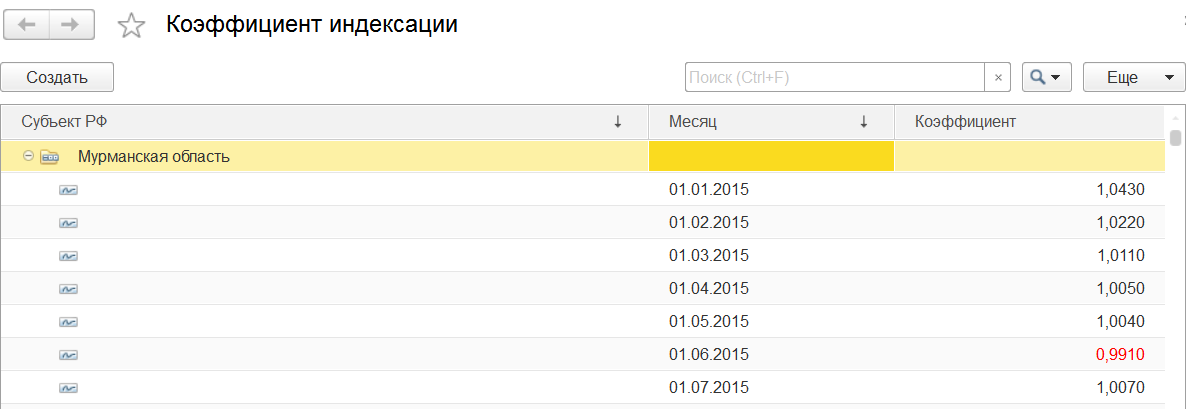
\includegraphics[scale=0.5]{ind7}}
\caption{Регистр сведений <<Коэффициенты индексации>>}
\label{ris:ind7}
\end{figure}

Коэффициенты вносятся для каждого месяца, участвующего в расчете, и в разрезе субъектов РФ, так как для каждого субъекта эти коэффициенты определяются в разном размере. Для удобства просмотра и редактирования значения коэффициентов сгруппированы по регионам и значения по ненужным регионам могут быть свернуты.

В случае, если по какому-то из месяцев коэффициент индексации меньше единицы (что соответствует отрицательному росту цен, зафиксированному Росстатом) --- он выделяется красным цветом.
\subsection{Пример, используемый для расчета индексации}
Истец Сидорова обратилась к мировому судье с иском на предмет взыскания не\-ус\-тойки по алиментам с бывшего мужа Кузнецова за период с 01~января 2014 года по 30~ноября 2014 года.

26 января 2015 года мировым судьей было постановлено решение - взыскать с Кузнецова в пользу Сидоровой неустойку по алиментам в размере 69~223~рублей 01~копейки.

01 декабря 2015 года Кузнецова обратилась к мировому судье с заявлением об индексации присужденных сумм, в котором просила взыскать сумму индексации присужденных сумм за период с 27 января 2015 года по 30 ноября 2015 года включительно. В заявлении указала, что с должника 15 июля 2015 года была принудительно взыскана сумма в размере 21 рубль 17 копеек, которая была направлена во исполнение данного решения; в остальной части решение остается неисполненным.

Дополнительно к этому, Кузнецова уже обращалась с заявлением об индексации присужденных сумм: определением от 22 апреля 2015 года в её пользу уже была взыскана индексация за период с 27 января 2015 года по 31 марта 2015 года в размере 2~796~рублей 61~копейки.
\subsection{Последовательность заполнения документа}
Основное окно документа представлено на рисунке \ref{ris:ind1}.
\begin{figure}[h]
\center{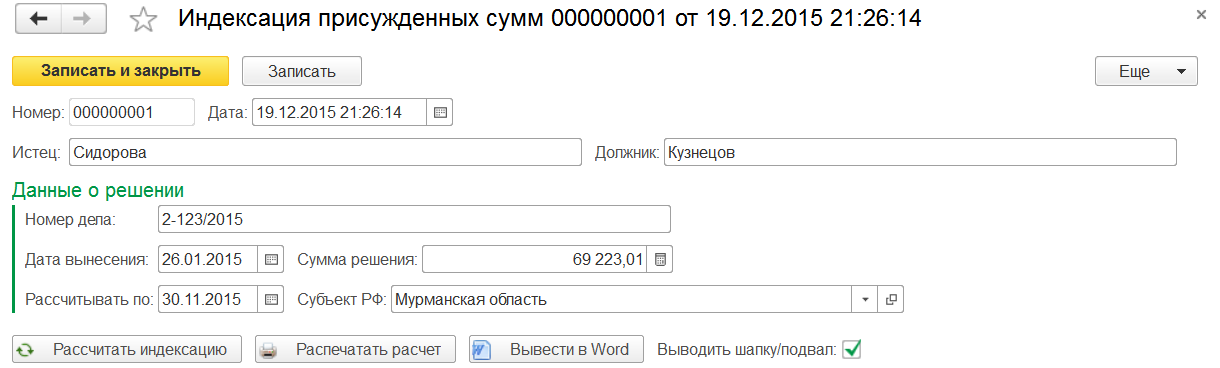
\includegraphics[scale=0.5]{ind1}}
\caption{Окно документа <<{\it Индексация присужденных сумм}>>}
\label{ris:ind1}
\end{figure}

Можно заметить, что многие поля, относящиеся к судебному решению совпадают, по названию и смыслу, с полями документа <<{\it Неустойка по алиментам}>>. Однако, дополнительно к ним, обязательным является заполнение полей <<{\it Дата вынесения}>>, <<{\it Сумма решения}>> и <<{\it Рассчитывать по}>> --- если данные поля не заполнены, то расчет индексации выдаст пользователю ошибку.

Далее, принципиально важным для правильного исчисления сумм индексации является заполнение поля <<{\it Субъект РФ}>> --- в случае, если данное поле не заполнено, то коэффициенты индексации будут браться по субъекту Федерации, установленному по умолчанию в настройках программы; в итоге это может привести к завышению или занижению суммы индексации.

Флаг <<{\it Включать в расчет дату вынесения}>> по умолчанию выключен. Однако, если его включить, то расчетный период будет отсчитываться не от дня, следующего за вынесением судебного решения, а с даты вынесения; таким образом, индексация будет рассчитана за +1 день.

В случае, если в расчетном периоде судебное решение исполнялось, необходимо отразить в таблице <<{\it Оплаты}>> соответствующие даты и суммы (рисунок \ref{ris:ind2}):
\begin{figure}[h]
\center{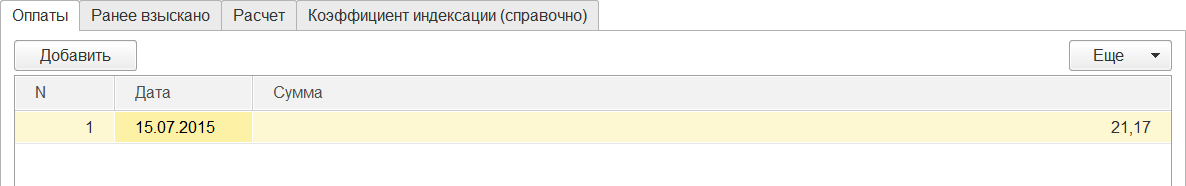
\includegraphics[scale=0.5]{ind2}}
\caption{Таблица <<{\it Оплаты}>>}
\label{ris:ind2}
\end{figure}

Далее, касательно нашего примера, в таблице <<{\it Ранее взыскано}>> необходимо отразить, что взыскатель уже обращался за индексацией ранее, чтобы эти суммы были учтены в окончательном расчете (рисунок \ref{ris:ind3}):

\begin{figure}[h]
\center{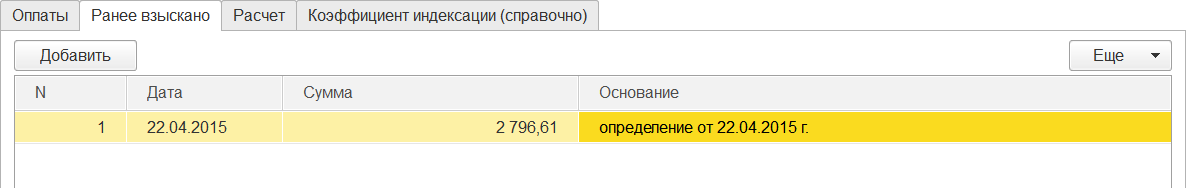
\includegraphics[scale=0.5]{ind3}}
\caption{Таблица <<{\it Ранее взыскано}>>}
\label{ris:ind3}
\end{figure}

В случае, если заполнена шапочная часть документа со сведениями о судебном решении и (при необходимости) таблицы <<{\it Оплаты}>> и/или <<{\it Ранее взыскано}>>, можно произвести расчет индексации нажатием соответствующей кнопки.

При этом заполняются таблицы<<{\it Расчет}>> (рисунок \ref{ris:ind4}) и <<{\it Коэффициенты индексации (справочно)}>> (рисунок \ref{ris:ind5}). Необходимо отметить, что их заполнение производится полностью автоматически и для редактирования обе эти таблицы недоступны.

\begin{figure}[h]
\center{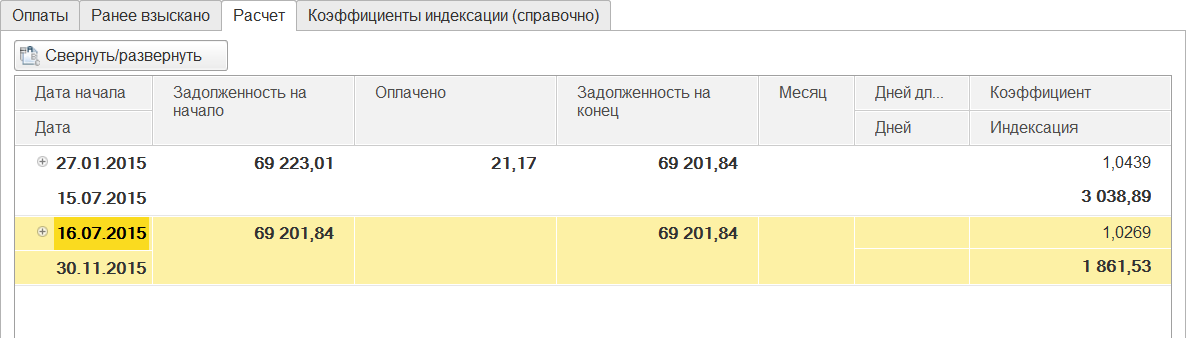
\includegraphics[scale=0.5]{ind4}}
\caption{Таблица <<{\it Расчет}>>}
\label{ris:ind4}
\end{figure}
\begin{figure}[h]
\center{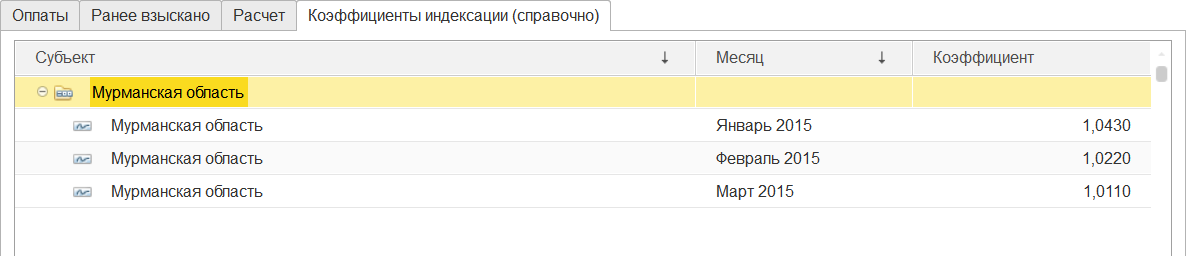
\includegraphics[scale=0.5]{ind5}}
\caption{Таблица <<{\it Коэффициенты индексации (справочно)}>>}
\label{ris:ind5}
\end{figure}

Стоит обратить внимание на то, что таблица <<{\it Расчет}>> имеет специальный вид, а именно, она является двухуровневой. На первом уровне строк у нас выведены общие суммы индексации за подпериоды, соответствующие датам исполнения судебного решения, а на втором уровне подсчитывается количество дней и коэффициенты индексации для каждого месяца, входящего в период расчета полностью или частично. 

При необходимости таблица <<{\it Расчет}>> может быть развернута полностью нажатием кнопки <<{\it Свернуть/развернуть}>>, а повторное нажатие возвращает таблицу в исходный (компактный) вид.

Можно заметить, что таблица на рисунке \ref{ris:ind5} весьма похожа на окно регистра сведений <<{\it Коэффициенты индексации}>> (см. раздел \ref{sec:rs_ind}). Это неудивительно --- на самом деле это одна и та же форма, просто в данном случае на неё наложены ограничения: выводятся только те коэффициенты, которые актуальны для нашего конкретного документа.

Окончательно, аналогично документу <<{\it Неустойка по алиментам}>>, после произведения расчета возможно распечатать печатную форму расчета индексации либо вывести её в Microsoft Word, при этом также остается возможность флагом <<{\it Выводить шапку/подвал}>> регулировать вывод в форму расчета справочной части расчета со сведениями о судебном решении (рисунок \ref{ris:ind6}):
\begin{figure}[h]
\center{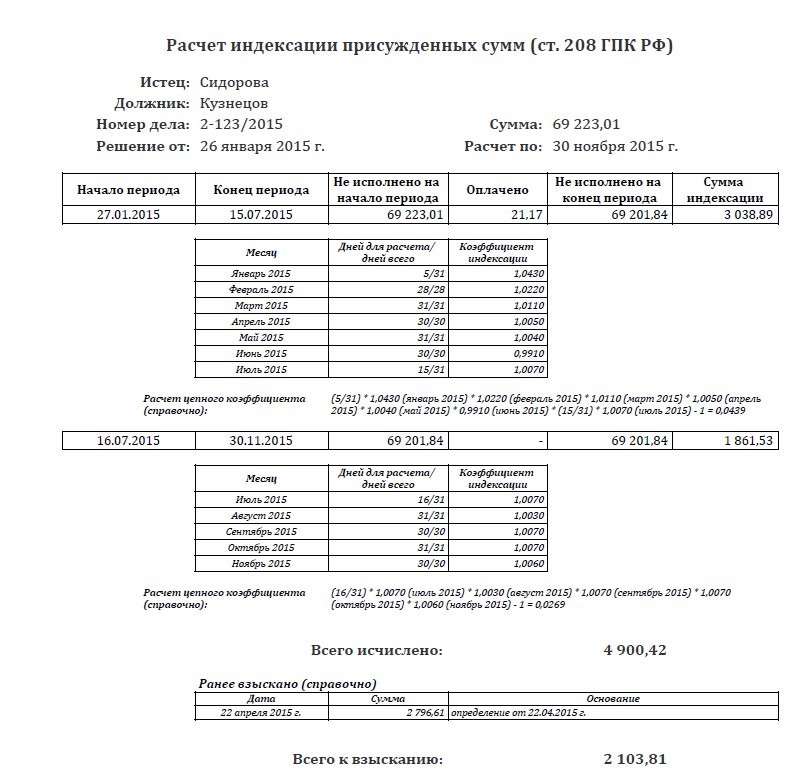
\includegraphics[scale=0.8]{ind6}}
\caption{Печатная форма расчета индексации}
\label{ris:ind6}
\end{figure}
\clearpage
\section{Документ <<Проценты за пользование денежными средствами>>}

Взыскание процентов за пользование денежными средствами является универсальной мерой гражданско-правовой ответственности за неправомерное пользование денежными средствами вследствие неисполнения денежного обязательства, предусмотренной статьей 395 Гражданского Кодекса РФ.

Право на получение данных процентов может возникнуть у взыскателя во многих случаях, когда денежное обязательство возникает в силу договора или закона --- например, при взыскании процентов за несвоевременную оплату поставленных товаров или выполненных работ/услуг, уклонение от возврата займа, невозврат полученного неосновательного обогащения и т.д.

Следует заметить, что исчисление данных процентов имеет свои особенности, как в части расчета процентной ставки, так и в части исчисления сроков.

В частности, право на начисление процентов за пользование денежными средствами возникает у кредитора начиная со дня, следующего за сроком исполнения денежного обязательства, и начисление продолжается до момента оплаты, при этом день оплаты также включается в расчет. При этом не усматривается невозможности применения этих принципов и для случая неоднократного увеличения задолженности в разные сроки (допустим, для случая периодического платежа), и для случаев частичной оплаты по денежному обязательству.

Для расчетных периодов, имевших место до 01 июня 2015 года, в качестве расчетной процентной ставки принимается ставка рефинансирования Банка России, а для периодов начиная с 01 июня 2015 года ставка является дифференцированной в зависимости от места жительства\footnote{Следует принять во внимание, что Банк России публикует настоящую ставку в разрезе федеральных округов РФ} кредитора (или юридического адреса кредитора, являющегося юридическим лицом) и равна опубликованной Банком России средней ставке банковского процента по вкладам физических лиц.

Далее, согласно позиции высших судов\footnote{п. 2 совместного Постановления Пленума Верховного Суда РФ № 13, Пленума ВАС РФ № 14 от 08~октября 1998 года <<О практике применения положений Гражданского кодекса Российской Федерации о процентах за пользование чужими денежными средствами>>} при расчете сроков календарный год принимается равным 360 дням и состоящим из 12 месяцев, каждый из которых состоит из 30 дней.

\subsection{Пример, используемый для заполнения документа}
01 декабря 2015 года Зайцев обратился к мировому судье с иском на предмет взыскания задолженности по договору займа с Волкова.

В обоснование иска истец указал, что между ним и ответчиком был заключен договор займа, в соответствие с которым Зайцев 31 декабря 2014 года выдал Волкову займ в размере 30~000 рублей, а Волков обязался погасить займ тремя частями по 12~000 рублей не позднее, соответственно, 31 марта, 30 июня и 30 сентября 2015 года.

Однако полное погашение в соответствие с условиями данного графика Волков не произвел, были произведены два перечисления --- 5~000 рублей 01 мая 2015 года и 4~000 рублей 15 сентября 2015 года.

Согласно изложенному, Зайцев просит взыскать с Волкова остаток долга по договору займа в размере 27~000 рублей и проценты за пользование денежными средствами за период с 01 апреля 2015 года по 30 ноября 2015 года включительно.

Как усматривается из обстоятельств дела, ответчиком допущена просрочка исполнения денежного обязательства из договора займа, начиная с 01 апреля 2015 года. Следовательно, в период с 01 апреля 2015 года по 31 мая 2015 года необходимо исчислить сумму процентов за пользование, исходя из ставки рефинансирования, а с 01 июня 2015 года по 30 ноября 2015 года --- исходя из средней ставки банковского процента по вкладам физлиц.

Для определенности будем считать, что в спорном периоде Зайцев постоянно проживал на территории Северо-Западного федерального округа.
\subsection{Заполнение документа}

Заполнение документа <<{\it Проценты за пользование денежными средствами}>> во многом аналогично заполнению документов, рассмотренных ранее в настоящем руководстве, однако правильная настройка расчета в нём важна и имеет свою специфику.

Рассмотрим заголовочную часть документа:
\begin{figure}[h]
\center{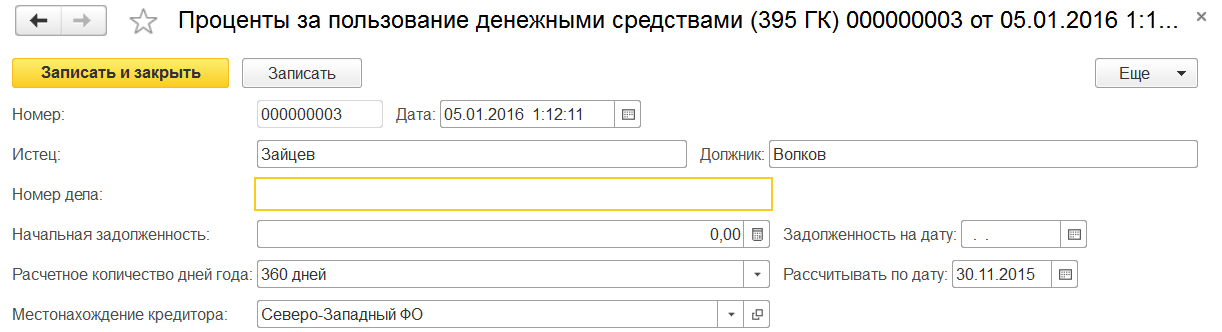
\includegraphics[scale=0.5]{pp1}}
\caption{Документ <<{\it Проценты за пользование денежными средствами}>>}
\label{ris:pp1}
\end{figure}

Назначение некоторых полей по сравнению с прошлым документами не меняется, поэтому детально рассмотрим только поля, которые специфичны именно для этого вида документов.

Первым существенным отличием является наличие пары полей <<{\it Начальная задолженность}>> и <<{\it Задолженность на дату}>>. В нашем примере они не заполнены, однако в случае, если расчет необходимо производить с учетом некоторой входящей задолженности на некоторую дату, то эти поля заполняются в обязательном порядке. С целью избежать ошибок при заполнении одного из полей (суммы или даты) второе поле становится обязательным для заполнения автоматически.

Далее, конечная дата периода расчета, включительно по которую он будет производиться, задается в поле <<{\it Рассчитывать на дату}>>. Так как период расчета в любом случае должен быть ограничен --- заполнение этого поля является строго обязательным.

Поле выбора <<{\it Расчетное количество дней года}>> определяет порядок пересчета расчетной ставки, выраженной в годовых процентах, в процент за день. В зависимости от выбранного варианта, деление годовой величины процента будет производиться календарно (на 365 дней) либо согласно ППВС № 13 от 08.10.1998 г. (на 360 дней).

Заканчивается заполнение заголовочной части документа выбором  в поле <<{\it Местонахождение кредитора}>> федерального округа по месту нахождения истца-кредитора из соответствующего списка. Необходимо отметить, что данное поле становится видимым только в случае, когда датой окончания расчета является дата после 01 июня 2015 года --- начиная с этой даты при расчете процентов за пользование применяется средняя ставка процентов по вкладам физических лиц, различающаяся по федеральным округам.

В случае, если нам необходимо рассчитать проценты за пользование денежными средствами в случае, когда сумма применяемой для расчета задолженности во времени меняется ввиду начислений или частичных погашений, дополнительно к заголовочной части документа должны быть заполнены таблицы документа во вкладках <<{\it Начисления}>> (рис. \ref{ris:pp2}) и <<{\it Платежи}>> (рис. \ref{ris:pp3}).

Для правильного заполнения таблицы начислений важно понимать, что в графе <<{\it Срок оплаты}>> указывается именно срок оплаты, т.е. последняя дата, в которую соответствующий периодический платеж ещё не является просроченным. При расчете период просрочки будет автоматически исчисляться от дня, следующего за очередным сроком оплаты.

\begin{figure}[h]
\center{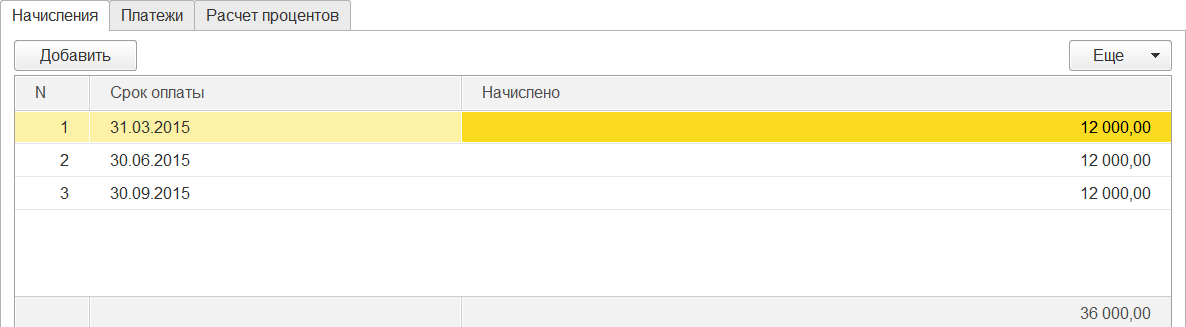
\includegraphics[scale=0.5]{pp2}}
\caption{Таблица <<{\it Начисления}>>}
\label{ris:pp2}
\end{figure}

\begin{figure}[h]
\center{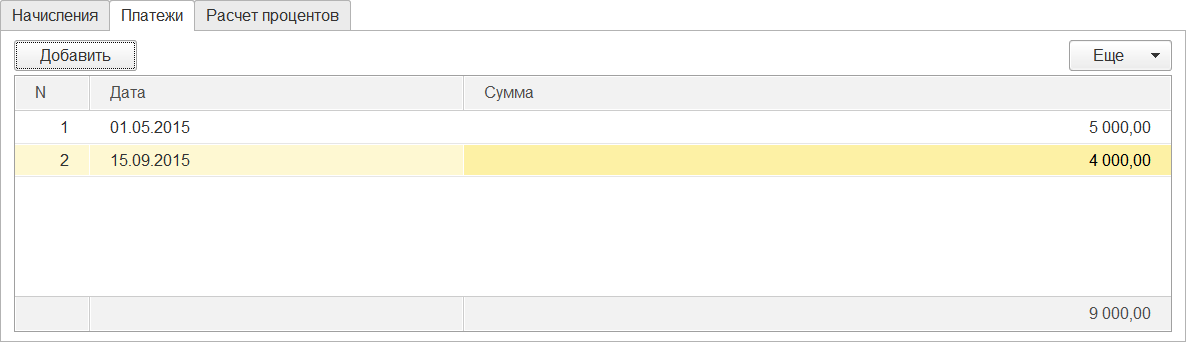
\includegraphics[scale=0.5]{pp3}}
\caption{Таблица <<{\it Платежи}>>}
\label{ris:pp3}
\end{figure}

Дополнительно, в целях проверки вводимых данных, в случае, если срок оплаты или дата платежа превышает конечную дату расчета --- значение в поле <<{\it Рассчитывать на дату}>> --- либо предшествует дате начальной задолженности --- значению в поле <<{\it Задолженность на дату}>>, если оно заполнено --- соответствующая строка выводится перечеркнутой и в расчете не участвует.

После того, как внесены все необходимые данные --- можно воспользоваться кнопкой <<{\it Рассчитать проценты}>>, при этом заполнится третья вкладка документа с таблицей <<{\it Расчет процентов}>>:
\begin{figure}[h]
\center{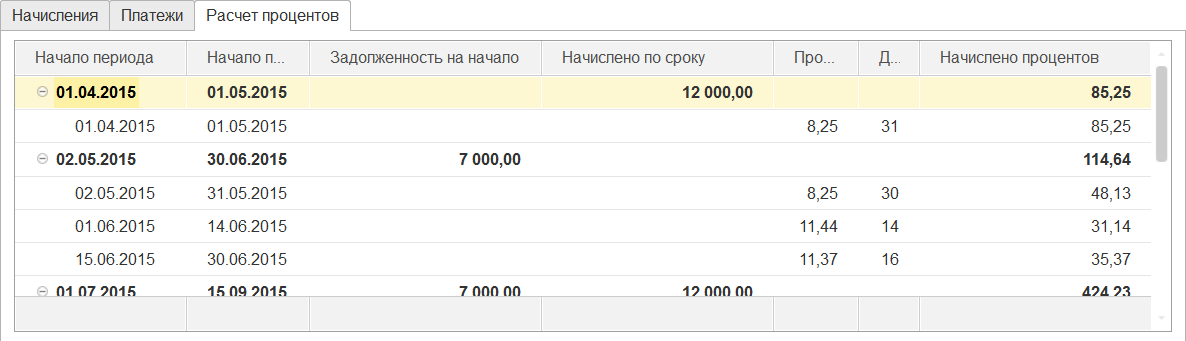
\includegraphics[scale=0.5]{pp4}}
\caption{Таблица <<{\it Расчет процентов}>>}
\label{ris:pp4}
\end{figure}

Как видно из рисунка, строки этой таблицы расположены в два уровня:
\begin{enumerate}
\item на первом уровне находятся периоды, соответствующие начислениям и оплатам, т.е. изменениям задолженности по денежному обязательству, от которой производится расчет процентов;
\item на втором уровне период детализируется далее --- он делится на составляющие периоды в зависимости от того, происходило ли в периоде уровня 1 изменение расчетной процентной ставки; конкретный расчет суммы процентов за пользование производится именно здесь, затем сумма по низлежащим периодам уровня 2 подытоживается в периоде уровня 1.
\end{enumerate}

\end{document}<<{\it Рассчитывать на дату}>>